\documentclass[10pt,a4paper]{article}
\usepackage[latin1]{inputenc}
\usepackage{amsmath}
\usepackage{amsfonts}
\usepackage{amssymb}
\usepackage{epstopdf}
\usepackage[numbers, sort&compress]{natbib}
\usepackage{graphicx}
\author{Nayef Al-Saud}
\title{AR Keyboard}
\begin{document}
\newcommand{\fig}{fig. }
\maketitle
\begin{abstract}

\end{abstract}

\tableofcontents

\section{Introduction}\label{sec:Introduction}

\section{Color-spaces and information storage for computer vision processing}\label{sec:ColorSpacesAndInfoStorageForComputerVisionProcessing}

\subsection{Overview of ColorSpaces}\label{sec:OverviewOfColorSpaces}

No need for full probabilistic treatment; we're just looking for skin color, no pattern recognition. It's a complexity which isn't necessary for us, since we're trying to develop a color space which detects the skin while discarding anything pertaining to everything else. We're not trying to classify the image based on the pixel colors in the image. (M Jones Paper.)



\subsubsection{LAB}\label{sec:LAB}


\subsubsection{RGB}\label{sec:RGB}

\subsubsection{HSV}\label{sec:HSV}

\subsubsection{YCbCr}\label{sec:YCbCr}



\subsection{Constructing a New Color Space}\label{sec:ConstructingANewColorSpace}

In order to construct a new color space, we need to consider the coordinate system of the new color space, the orientation of the new color space, and the fidelity of the discrete representation of the axes.

The first consideration is most easily decided; because there's little obvious advantage otherwise, we choose a Cartesean coordinate system as this allows for a straightforward transformation involving only rotation, translation and scaling. Because we're interested in the color information in the image, it's useful to design the color space so there is a luminosity axis. This choice determines two of three rotational degrees of freedom, as will be discussed below.

As for the discrete representation of the axes, it's desired that all the information captured pertaining to a hand should be preserved; all other information is irrelevant. However, here we'll consider only the effect of a rotation and scaling on the discrete representation.


\subsubsection{Camera RGB and Normalization for Discrete Range}\label{sec:CameraRGB}



Due to the hardware being locked down at the application level, we do not have access to the raw camera feed. We do, however, have access to the compressed, post-processing 8-bit RGB image data. The processing involves evening up the color channel senors' sensitivity by way of multiplying each channel by an appropriate correction factor. This is partly why cameras likely have a 10 or 12 bit/channel capture rate, but after accounting for differences in sensitivity, it only outputs in 8-bit color depth.

The three-color RGB channel sensors commonly found in CCD cameras are based on how the human eye perceives colors. But in physical reality, light is actually hitting the camera as a continuous spectrum. Since it's impossible to map an infinite set of gaussians to it, we instead use some function which, for any frequency, will give the intensity of the light hitting the point at that frequency. This function is expanded in the basis set of three gaussians with mean values centered on the RGB frequencies. This model is used in cameras because the main purpose of cameras -- until recent times -- has been to capture images for human viewing. And while the RGB gaussian basis model is perfectly suited for capturing all the scene information which humans can perceive, it is not a complete representation.

Because we're searching for particular points in the real color space -- which, being a continuous function, is infinite dimensional -- there is a possibility in the future that larger multi-channel color spaces will be much more common, such as the 8-channel color spaces currently in development. Though most such cameras are primarily designed for post-production editing for still pictures and film (e.g. changing the lighting independent of the scene), as well as visual effects, the possibilities for computer vision are exciting. However, computer vision tasks are computationally intensive, and more often than not require operation in real time, so there is a natural inclination to shy away from large data sets in practical computer vision applications; many tasks are done in grayscale or single channel processing to expedite the process.

As such, there is a need to develop techniques which keep the relevant information while quickly and efficiently discarding the irrelevant information. This is true for the RGB space at the moment, and the aim of this first part of the work.


\subsubsection{Rotation Matrix}\label{sec:RotationMatrix}

Any rotation about an axis can be represented by a matrix. Such rotations can be expressed as a 3x3 square matrix in a 3D space. Since they are generally invertible, they're guaranteed to be non-singular. For this application, we require rotation about three different axes, which can be expressed thus:


\begin{alignat}{1}
R_x(\theta) &= \begin{bmatrix}
1 & 0 & 0 \\
0 & \cos \theta &  -\sin \theta \\[3pt]
0 & \sin \theta  &  \cos \theta \\[3pt]
\end{bmatrix} \\[6pt]
R_y(\theta) &= \begin{bmatrix}
\cos \theta & 0 & \sin \theta \\[3pt]
0 & 1 & 0 \\[3pt]
-\sin \theta & 0 & \cos \theta \\
\end{bmatrix} \\[6pt]
R_z(\theta) &= \begin{bmatrix}
\cos \theta &  -\sin \theta & 0 \\[3pt]
\sin \theta & \cos \theta & 0\\[3pt]
0 & 0 & 1\\
\end{bmatrix}
\end{alignat}


It should be noted that the solutions are not unique; there are many ways in which to rotate an object from one position to another, or use a combination of different rotations to get to the same point, so they aren't necessarily unique, but this has no bearing on this project. So any rotation which orients the RGB color space such that one of the new axes lies along the luminosity direction is sufficient. To achieve this end using rotations about the RGB color space axes requires a rotation in only two of those axes.

A rotation which aligns the X axis along the luminosity direction is produced by a rotation of $\frac{\pi}4$ about the Y axis, followed by a rotation of $\arctan{\frac{1}{\sqrt{2}}}$ about the Z axis. This leaves one free rotational degree of freedom about the X axis. The resulting rotation matrix is given by:

\begin{equation}
R_{xyz}(\theta) =
\left(
\begin{array}{ccc}
 \frac{1}{3} & \frac{1}{3} & \frac{1}{3} \\
 -\frac{\cos (\theta )}{2}-\frac{1}{2} \sqrt{3} \sin (\theta ) & \cos (\theta ) & \frac{1}{2} \sqrt{3} \sin (\theta )-\frac{\cos (\theta )}{2} \\
 \frac{\sin (\theta )}{2}-\frac{1}{2} \sqrt{3} \cos (\theta ) & -\sin (\theta ) & \frac{1}{2} \sqrt{3} \cos (\theta )+\frac{\sin (\theta )}{2} \\
\end{array}
\right)
\end{equation}


Where $\theta$ is the remaining rotational degree of freedom.

Using the standard rotation matrices, we get a luminosity axis from 0 to $\sqrt{3}$. However, the length of the two remaining axes are dependent on the value of $\theta$ used. This is a problem because, ultimately, we want the axes to fit in a range of an appropriate data type. It would be more useful to have a matrix which provided the specified rotation and scaled the axis to known lengths. In the case of the luminosity, this is straightforward; simply divide by $\sqrt{3}$. In the case of the other two axes, we need an explicit form for the lengths of the axis resulting from the rotation.

Because the absolute values of the axes in the color space have no meaning, we're only interested in the position along the axis relative to its start and end, equivalent to talking about the position in the axis relative to 0 to 1, compared to about 0-255 in unsigned, 8-bit integers. The upside is that if we're rotating the cube about its corner, we're interested in the minimum and maximum values possible along the new axis direction, which will correspond to a corner of the RGB cube. With the X axis aligned along the luminosity direction, the range of the X axis is 0 to $\sqrt{3}$. The Y and Z axes are symmetrical, spanning a range centered on 0. The range of their values is dependent upon the remaining degree of freedom.

We need to know, in each of the axes, how far out each point is. Because we're effectively rotating a hexagon, whatever the answer is, we know the function is going to be periodic, repeating every $\frac{\pi}{3}$ radians, so we only have to solve it in the 0 to $\frac{\pi}{3}$ region and then generalize. First we take the cooordinates of the RGB cube and perform the rotation to find the values in the new color space.

\begin{multline}\label{YabCube}
  R_{xyz}(\theta)\cdot\left(
\begin{array}{cccccccc}
 0 & 1 & 1 & 0 & 0 & 0 & 1 & 1 \\
 0 & 0 & 1 & 1 & 1 & 0 & 0 & 1 \\
 0 & 0 & 0 & 0 & 1 & 1 & 1 & 1 \\
\end{array}
\right) = \\
\left(
\begin{array}{cccccccc}
 0 & \frac{1}{\sqrt{3}} & \frac{2}{\sqrt{3}} & \frac{1}{\sqrt{3}} & \frac{2}{\sqrt{3}} & \frac{1}{\sqrt{3}} & \frac{2}{\sqrt{3}} & \sqrt{3} \\
 0 & -\frac{\cos (\theta)}{\sqrt{6}}-\frac{\sin (\theta)}{\sqrt{2}} & \frac{\cos (\theta)}{\sqrt{6}}-\frac{\sin (\theta)}{\sqrt{2}} & \sqrt{\frac{2}{3}} \cos (\theta) & \frac{\cos (\theta)}{\sqrt{6}}+\frac{\sin (\theta)}{\sqrt{2}} & \frac{\sin (\theta)}{\sqrt{2}}-\frac{\cos (\theta)}{\sqrt{6}} & -\sqrt{\frac{2}{3}} \cos (\theta) & 0 \\
 0 & \frac{\sin (\theta)}{\sqrt{6}}-\frac{\cos (\theta)}{\sqrt{2}} & -\frac{\cos (\theta)}{\sqrt{2}}-\frac{\sin (\theta)}{\sqrt{6}} & -\sqrt{\frac{2}{3}} \sin (\theta) & \frac{\cos (\theta)}{\sqrt{2}}-\frac{\sin (\theta)}{\sqrt{6}} & \frac{\cos (\theta)}{\sqrt{2}}+\frac{\sin (\theta)}{\sqrt{6}} & \sqrt{\frac{2}{3}} \sin (\theta) & 0 \\
\end{array}
\right)
\end{multline}

The extent of the new axis is found by taking the maximum and minimum values of each row i.e. the extreme corner positions relative to each new axis. An additional symmetry of the hexagonal projection of the RGB cube allows us to say that whatever functional form is taken by one of the $\theta$ dependant ranges the other can be found by a simple phase shift. So recognising that the minimum value is simply $-1$ times the maximum we have simplified the problem to solving

\begin{equation}\label{AxisRangeMinMax}
 \max\left(\pm\frac{\sin (\theta )}{\sqrt{6}}\pm\frac{\cos (\theta )}{\sqrt{2}}, \pm\sqrt{\frac{2}{3}} \sin (\theta ) \right) \quad \text{Where} \quad 0\leq \theta \leq \frac{\pi}{3}
\end{equation}

Graphically, the problem appears as follows:

\includegraphics{YABCubeEval.eps}

In the range 0 to $\frac{\pi}{3}$, both sin and cos are positive, therefore the axis ranges are given by the following:

\begin{tabular}{|c|c|c|}
  \hline
  % after \\: \hline or \cline{col1-col2} \cline{col3-col4} ...
    & Min & Max \\ \hline
  X & \(0\) & \(\sqrt{3}\) \\
  Y & \(-\frac{\sin \left((\left(\theta -\frac{\pi }{6}\right) \bmod \frac{\pi }{3})\right)}{\sqrt{6}}-\frac{\cos \left((\left(\theta -\frac{\pi }{6}\right) \bmod \frac{\pi }{3})\right)}{\sqrt{2}}\) & \(\frac{\sin \left((\left(\theta -\frac{\pi }{6}\right) \bmod \frac{\pi }{3})\right)}{\sqrt{6}}+\frac{\cos \left((\left(\theta -\frac{\pi }{6}\right) \bmod \frac{\pi }{3})\right)}{\sqrt{2}}\) \\
  Z & \(-\frac{\sin \left((\theta  \bmod \frac{\pi }{3})\right)}{\sqrt{6}}-\frac{\cos \left((\theta  \bmod \frac{\pi }{3})\right)}{\sqrt{2}} \) & \(\frac{\sin \left((\theta  \bmod \frac{\pi }{3})\right)}{\sqrt{6}}+\frac{\cos \left((\theta  \bmod \frac{\pi }{3})\right)}{\sqrt{2}}\) \\
  \hline
\end{tabular}

It is convenient to produce a transformation which will result in axes of known length. Because the rotation cannot include a translation, we desire a transformation matrix which will result in the ranges 0 to 1, -$\frac{1}2$ to $\frac{1}2$, and -$\frac{1}2$ to $\frac{1}2$. Such a transformation is easily obtained by multiplying the rotation matrix by a diagonal matrix with the reciprocal of the maximums found above placed along the diagonal. This will scale each axis to a unit length.

The normalised rotation matrix is given by:

\begin{equation}\label{NormRxyz}
R_{xyz}(\theta) = \left(
\begin{array}{ccc}
 \frac{1}{3} & \frac{1}{3} & \frac{1}{3} \\
 -\frac{\sqrt{3} \cos (\theta )+3 \sin (\theta )}{3 \cos \left((\left(\theta +\frac{\pi }{6}\right) \bmod \frac{\pi }{3})\right)+\sqrt{3} \sin \left((\left(\theta +\frac{\pi }{6}\right) \bmod \frac{\pi }{3})\right)} & \frac{2 \sqrt{3} \cos (\theta )}{3 \cos \left((\left(\theta +\frac{\pi }{6}\right) \bmod \frac{\pi }{3})\right)+\sqrt{3} \sin \left((\left(\theta +\frac{\pi }{6}\right) \bmod \frac{\pi }{3})\right)} & \frac{3 \sin (\theta )-\sqrt{3} \cos (\theta )}{3 \cos \left((\left(\theta +\frac{\pi }{6}\right) \bmod \frac{\pi }{3})\right)+\sqrt{3} \sin \left((\left(\theta +\frac{\pi }{6}\right) \bmod \frac{\pi }{3})\right)} \\
 \frac{\sqrt{3} \sin (\theta )-3 \cos (\theta )}{3 \cos \left((\theta  \bmod \frac{\pi }{3})\right)+\sqrt{3} \sin \left((\theta  \bmod \frac{\pi }{3})\right)} & -\frac{2 \sqrt{3} \sin (\theta )}{3 \cos \left((\theta  \bmod \frac{\pi }{3})\right)+\sqrt{3} \sin \left((\theta  \bmod \frac{\pi }{3})\right)} & \frac{3 \cos (\theta )+\sqrt{3} \sin (\theta )}{3 \cos \left((\theta  \bmod \frac{\pi }{3})\right)+\sqrt{3} \sin \left((\theta  \bmod \frac{\pi }{3})\right)} \\
\end{array}
\right)
\end{equation}

\subsection{Skin Statistics}\label{sec:SkinStatistics}

In order to identify the range of values for the skin space, a large number of skin samples were taken from photographs from the Humane project by Angelica Dass, an ongoing "chromatic inventory" art project which aims to compile every possible human skin color, categorized by the PANTONE guide color classification system. The skin colors catalogued thus far are independent of race or ethnicity, so the samples are representative of human skin tones in general.

The image set consists of approximately 200 skin samples --- each of which shows only skin --- which are placed in a single directory in the file system. In accordance to our assumption that luminosity is not a significant factor in our skin model, we then perform the transformation initially with the value of $\theta$ equal to 0. The Matlab code collects frequency data for the rotated color space, incrementing the counts of a three-dimensional array of bins which span the color space. Viewing the frequency data along each of the three axes reveals that the skin image characteristics are spread widely in luminosity, but are quite confined in hue and saturation as illustrated below:


\begin{figure}[h!]
  \caption{Initial set of bins.}
  \centering
    \includegraphics[width=\textwidth]{InitialBins.eps}
\end{figure}


Aside from differing lighting, this is consistent with the notion that skin has a distinct pigmentation and justifies our attempt to find an appropriate color space disregarding luminosity. In doing so, the distribution of the skin color characteristics neatly fit into a 2-dimensional Gaussian distribution. The Matlab code produces a fit with a 2-dimensional Gaussian distribution and provides an angle relative to the orientation of the Gaussian fit to the skin sample distribution in the current color space. 

Given that we are free to choose the orientation of the color space about the luminosity axis, the Matlab code allows us to find an orientation $\theta$ of the color space about the luminosity axis in which the distribution can be expressed as a product of 1-dimensional Gaussians along the axes. The final resulting distribution is presented in Figure~\ref{fig:DistributionAndGaussianFit}.


\begin{figure}[h!]
  \caption{Distribution and Gaussian fit to the chromatic pixel values in the new color space.}
  \label{fig:DistributionAndGaussianFit}
  \centering
    \includegraphics[width=\textwidth]{crosshairFigureFinal.eps}
\end{figure}


For numerical reasons, the value for $\theta$ was found iteratively by performing the color space transformation and the statistical fit until the value for $\theta$ converged. (See Figure~\ref{fig:ConvergenceTheta}.)


\begin{figure}[h!]
  \caption{Convergence of color space orientation $\theta$.}
  \label{fig:ConvergenceTheta}
  \centering
    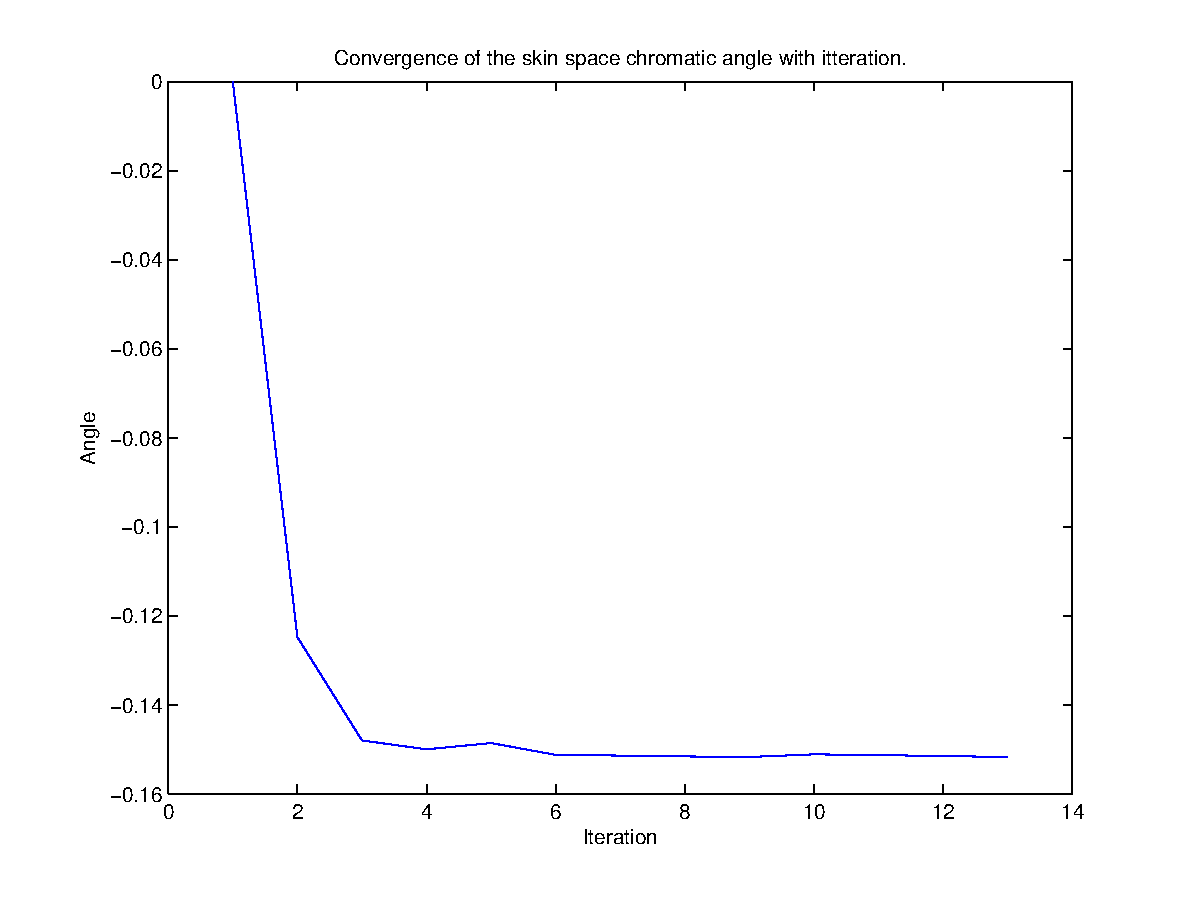
\includegraphics[width=\textwidth]{ConvergenceOfSkinSpaceFinal.eps}
\end{figure}





\begin{figure}[h!]
  \caption{Rainbowman in a stunning three colors plus the other thing.}
  \centering
    \includegraphics[width=\textwidth]{rainbowmanRGB.eps}
\end{figure}

\begin{figure}[h!]
  \caption{Rotated Rainbowman.}
  \centering
    \includegraphics[width=\textwidth]{rainbowmanRotated.eps}
\end{figure}

\begin{figure}[h!]
  \caption{Final bins.}
  \centering
    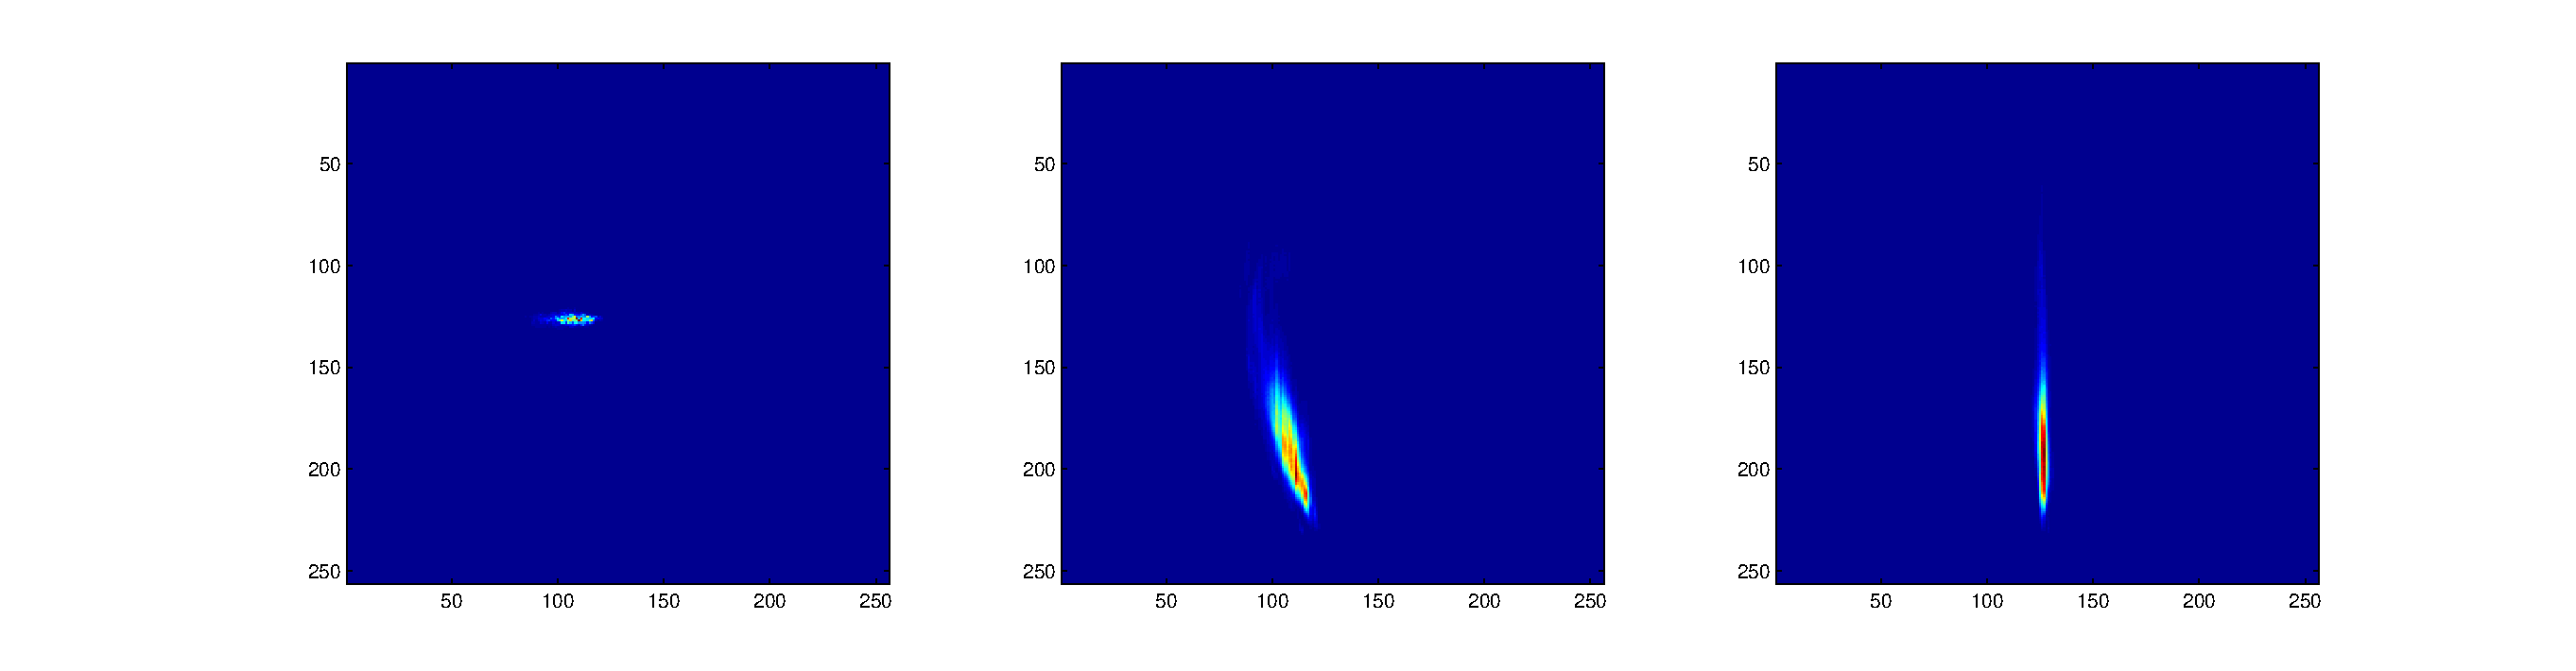
\includegraphics[width=\textwidth]{binsFinal2.eps}
\end{figure}

\begin{figure}[h!]
  \caption{Rotated and scaled Rainbowman.}
  \centering
    \includegraphics[width=\textwidth]{rainbowmanRotatedScaled.eps}
\end{figure}

\begin{figure}[h!]
  \caption{Rotated compact scaled Rainbowman.}
  \centering
    \includegraphics[width=\textwidth]{rainbowmanRotatedCompactScaled.eps}
\end{figure}


\subsection{Preservation of Color Information}\label{sec:PreservationOfColorInformation}

The goal of the algorithm is to preserve all the information captured by the camera which relates to skin whilst discarding as much of the irrelevant information as possible. Given that edges and features often present as shadows and highlights, all the information captured in terms of luminosity will be regarded as relevant information, at least as far as the manipulation of individual pixel values is concerned. Considering the chromatic information, the importance of the pixel value will be directly determined by the Gaussian distribution found previously.

Knowing the range of values produced by the rotation allows us to scale the transformation to fit into the range of destination data type. If we have RGB pixel values in a given machine data type, the amount of information contained in each of those channels is equal to the number of values accessible in that data type. For example: for 8-bit, unsigned integers, there are 256 possible values. After a rotation, we are interested in the amount of information which lies along the new axes. This is found simply by multiplying the range of the source data type by the length of the new axes found for the unit cube. To preserve all the information captured, we would therefore have to use a larger data type to store the new values. We are, however, only interested in a small region in the chromatic space, at least. The question is, then, how to preserve the relevant information in a way consistent with the significance indicated by the Gaussian distribution found previously.

\begin{figure}[h!]
  \caption{Linear approximation.}
  \label{fig:Linear}
  \centering
    \includegraphics[width=0.49\textwidth]{linearSmooth.eps}
    \includegraphics[width=0.49\textwidth]{linearColor.eps}
\end{figure}

\begin{figure}[h!]
  \caption{Linear partition approximation.}
  \label{fig:Partition}
  \centering
    \includegraphics[width=0.49\textwidth]{partitionSmooth.eps}
    \includegraphics[width=0.49\textwidth]{partitionColor.eps}
\end{figure}

\begin{figure}[h!]
  \caption{Error Function approximation.}
  \label{fig:ERF}
  \centering
    \includegraphics[width=0.49\textwidth]{ERFSmooth.eps}
    \includegraphics[width=0.49\textwidth]{ERFColor.eps}
\end{figure}

\begin{figure}[h!]
  \caption{Unit graph.}
  \label{fig:UnitGraph}
  \centering
    \includegraphics[width=\textwidth]{unitGraph.eps}
\end{figure}


None of the rotated axes have lengths less than 1 for the unit RGB cube. For this reason we've written redistribution functions which perform any necessary type conversion whilst preserving the information in a controlled way; we can keep the information where it's needed and discard it where it's irrelevant. So although this is strictly beyond the normal meaning of a color space conversion, it is addressing a connected issue and belongs in the conversion. In terms of optimisation, it is also the most efficient place in the code in which to perform this adjustment, allowing us to --- for the sake of example --- discard the details of the colors of a duck's feathers whilst keeping the hues and tones of human skin.

We can use a function to redistribute the information contained on the longer axis onto the shorter axis, which can be expressed in the discrete representation of that axis necessitated by internal integer data types. There are three ways in which to implement the redistribution functions:

\subsubsection{Partition}\label{sec:Partition}
The most straightforward redistribution method is to simply preserve the information in a 1-to-1 fashion within a region. The region can be defined in terms of the skin color distribution Gaussian by specifying a significance level in terms of the variance or the standard deviation.

\subsubsection{Linear}\label{sec:Linear}
A slightly more sophisticated method is to use a linear redistribution. A linear distribution is equivalent to partitioning given a unit gradient. However, a linear redistribution function allows for the possibility of data compression. So then, in the case where the region of interest contains more information than can be expressed in the destination data type, a linear distribution function allows an even compression of the information from source to destination.

\subsubsection{ERF (Gaussian Error Function)}\label{sec:ERF}
The integral of the cumulative Gaussian (i.e. Error Function) allows the redistribution of the information on the axis in a way which selectively preserves the information about a point on the axis (i.e. the mean of the Gaussian), and then progressively discard the information as it falls into the tails of the Gaussian. So, it provides a non-linear distribution of the information. The Gaussian can be seen as describing our interest in the information contained along the axis, so it's logical to use the error function to redistribute the information. The disadvantage of this is simply the computational effort involved in generating the error function.

There are a variety of approximations to the error function. (Describe which one was chosen here.)


We will likely partition for the white/black axis, apply the linear redistribution for the distribution function on the axis which has the very low value of standard deviation, and the ERF for the axis which contains most of the variation for skin color.

(Insert graphs and data here)

\subsection{Setting up 2-Channel Representation}\label{sec:SettingUp2-ChannelRepresentation}
We've mathematically defined a method of distribution, but when observed in discrete terms, it's not an efficient packing of the information. One method of dealing with that is to use a lookup table. We do that where our continuous function spreads a unit interval over a larger range in the destination space. We can make the lookup table remove any jumps in it. It works with up to 8 bit numbers, because beyond that we get into massive tables, which isn't worth the effort. A way of mathematically implementing the same trick is to use a piecewise function, which behaves differently with different values. What we do is break the function into ranges (e.g. constant, ERF, linear, etc. depending on the gradient.) A linear dist is used when gradient is greater than 1, and back to the ERF when it goes down again. Const when nothing in particular's going on. Actually because it saves computational effort. (ERF gives same value; no point in doing it unnecessarily.) Doesn't fit full width of data type any more. (will be lower than max of data type; we squashed it.)

Another method of dealing with that is set the max grad in the ERF. Don't use piecewise, just use ERF and scale the destination so it fits. By dividing the max value by the max gradient of ERF (The ERF evaluated at center point.), it becomes more horizontal, until it has a grad of 1. Advantage is not dealing with piecewise function, mathematically consistent, disadvantage is that also squash out a lot of the ERF behavior and a lot of the info we wanted to keep on either side of that value. The only place it keeps info is bang in the center; everywhere else is losing info.

Finally we could compromise by finding the closest datatype which fits the amount of info into the retained range. It's not actually the amount of information that is retained, so it's accepting a bit of looseness in the data packing of that type, even if we found a perfect fit. For the datatype closest to info we want to retain, we then scale as in the second method.

The reason we're talking about bit depth and not byte depth (fitting into the closest power of 2) is that it allows us to easily combine with the bits in a second channel; fitting both channels into one data type. It's difficult to predict what it will look like, since we're combining two channels into one, but it's the most efficient way of combining the two, turning it into a one-channel problem. However, now two colors that were once close to each other will end up separated. Seeing as all the information is there, though, this may not matter. The question is if all the data is usable in this form.



\subsection{Skin Detection}\label{sec:SkinDetection}

\subsection{Putting it All Together}\label{sec:PuttingItAllTogether}

\subsection{Physiology Study}\label{sec:PhysiologyStudy}

\subsubsection{Pigment vs. Blood}\label{sec:PigmentVs.Blood}

\subsubsection{Blood Flow}\label{sec:BloodFlow}

\subsubsection{Apply the Effect}\label{sec:ApplyTheEffect}


\section{Pattern Recognition}\label{sec:PatternRecognition}


\subsection{Constant Patterns under Mechanical Stresses in the Hand}\label{sec:ConstantPatterns}
\subsection{Dynamic Patterns under Mechanical Stresses in the Hand}\label{sec:DynamicPatterns}
\subsubsection{Finger Pad Pressure}\label{sec:FingerPadPressure}
\subsubsection{Fingernail Pressure}\label{sec:FingernailPressure}
\subsection{Pattern Recognition Techniques in OpenCV}\label{sec:PaternRecognitionOpenCV}
\subsection{Implementation of Pattern Recognition using OpenCV on an iPhone}\label{sec:ImplementationOnIPhone}

\subsection{Refining the Target Area for Search}\label{sec:RefiningTargetAreaForSearch}
\subsubsection{Blob Detection}\label{sec:BlobDetection}
\subsubsection{Hand Posture Prediction}\label{sec:HandPosturePrediction}
\subsubsection{Dynamic Tracking}\label{sec:DynamicTracking}
\section{The Fingertip Mechanical Stress Detection App}\label{sec:FingertipMechanicalStressDetectionApp}
\subsection{OpenCV Integration with iOS}\label{sec:OpenCVIntegrationWithIOS}
\subsubsection{C++11 and OpenCV}\label{sec:C++11AndOpenCV}
\subsubsection{Integrating C++11, OpenCV and iOS Data Types}\label{sec:IntegratingC++11AndIOSDataTypes}
\subsubsection{Using Parallel Processing in OpenCV and iOS}\label{sec:ParallelProcessingInOpenCVAndIOS}
\subsubsection{Implementing Working Data Types Efficiently in OpenCV}\label{sec:ImplementingDataTypesEfficientlyOpenCV}
\subsection{Dynamic vs. Static Statistics}\label{sec:DynamicVsStaticStatistics}
\subsubsection{Color Space Dynamically Updated Statistics}\label{sec:ColorSpaceDynamicallyUpdatedStatistics}
\subsubsection{Updating the Pattern Recognition Model for Specific Individuals}\label{sec:UpdatingPatternRecognitionModelForSpecificIndividuals}
\subsubsection{Updating the Mechanical Stress Models to Account for Environment}\label{sec:UpdatingMechanicalStressModelsToAccountForEnvironment}
\subsection{Balancing the processor load}\label{sec:BalancingTheProcessorLoad}
\subsubsection{Frame Rate Capture vs. Frame Processing Rate}\label{sec:FrameRateCaptureVsFrameProcessingRate}
\subsubsection{Background Processes}\label{sec:BackgroundProcesses}
\subsubsection{Updating the Hand Posture Model}\label{sec:UpdatingTheHandPostureModel}
\subsubsection{Updating the Color Space Model}\label{sec:UpdatingTheColorSpaceModel}
\subsubsection{Updating the Scene Background Model}\label{sec:UpdatingTheSceneBackgroundModel}


\section{Future Work and Discussion}\label{sec:FutureWorkAndDiscussion}


\bibliographystyle{unsrtnat}
\bibliography{ARKeyboard}


\end{document}
